\documentclass[11pt]{article}
\usepackage{amsmath}
%\usepackage{extsizes}
\usepackage{amsmath,amssymb,amsthm}
%\usepackage{omegavn,ocmrvn}
%\usepackage[utf8x]{inputenc}
\usepackage[utf8]{vietnam}

\usepackage{listings}
\lstset{language=Python}          % Set your language (you can change the language for each code-block optionally)
\usepackage[most]{tcolorbox}

\usepackage{longtable}
\usepackage{answers}
\usepackage{graphicx}
\usepackage{array}
\usepackage{pifont}
\usepackage{picinpar}
\usepackage{enumerate}
\usepackage[top=3.0cm, bottom=3.5cm, left=3.5cm, right=2.5cm] {geometry}
\usepackage{hyperref}



\newtheorem{thm}{Theorem}
\newtheorem{definition}{Định nghĩa}
\newtheorem{bt}{Câu}
\newcommand{\RR}{\mathbb R}
\Newassociation{sol}{Solution}{ans}
\newtheorem{ex}{Câu}
\renewcommand{\solutionstyle}[1]{\textbf{ #1}.}
\def\im{\mathrm{im}}
\def\tx{\tilde{x}}
\def\ty{\tilde{y}}

\begin{document}
% \noindent

\begin{tabular*}
	{\linewidth}{c>{\centering\hspace{0pt}} p{.7\textwidth}}
	Trường ĐHKHTN, ĐHQGHN & {\bf Học Kỳ 2 (2021-2022)}
	\tabularnewline
	K64 TTƯD - Thầy Hà Phi & {\bf Bài Tập Giải Tích Số \\ \today}
	% Exercises on pages 239, 240 Cheney/Kincaid are really nice
	\tabularnewline
	\rule{1in}{1pt}  \small  & \rule{2in}{1pt} %(Due date:)
	\tabularnewline
	%  \tabularnewline
	%  &(Đề thi có 1 trang)
\end{tabular*}




\begin{center}
	{\bf Bài Tập Lý Thuyết Điều Khiển Hệ Thống - No. 4 \\
	     Observability of linear systems}
\end{center}

\begin{bt} 
	Chuyển hệ điều khiển LTI cấp $n$ sau về hệ điều khiển cấp 1 với biến điều khiển $u$, biến trạng thái $x$ và xét tính quan sát được của hệ cấp 1 thu được. \\
	\begin{equation}
		x^{(n)} + \a_{n-1} x^{(n-1)} + \dots + \a_1 \dot{x} + \a_0 x = 
		u^{(n)} + \b_{n-1} u^{(n-1)} + \dots + \b_1 \dot{u} + \b_0 u \ . 
	\end{equation} 
\end{bt}

\begin{bt}
Các hệ thống sau có quan sát được hay không? Vì sao? \\
\noindent	
a) \textbf{Dạng chính tắc điều khiển được (controllability canonical form)}
	%
	\begin{align}
		\dot{x} &= \m{0 & 1 & &  & \\ &  \ddots & \ddots &  & \\ & & \ddots & \ddots &   \\&  &  & 0 & 1 \\ -\a_1 & -\a_2 & \dots & \dots & -\a_{r} } x + \m{0 \\ \vdots \\ \vdots \\ 0 \\ 1} u, \\
		y &= \m{\b_1 &  \dots & \dots & \b_r} x + D u, 
	\end{align}
	%
	trong đó $\a_i$, $\b_i$, $D$ là các hệ số (thực hoặc phức). \\
\noindent	b) \textbf{Dạng chính tắc quan sát được (observability canonical form)}
	%
	\begin{align}
		\dot{x} &= \m{-\a_1 & 1 & &  & \\ \vdots &   & \ddots &  & \\ \vdots & & & \ddots &   \\ -\a_{r-1} &  &  &  & 1 \\ -\a_{r} & 0 & \dots & \dots & 0} x + \m{\b_1 \\  \vdots \\ \vdots \\ \b_{r-1} \\ \b_r} u, \\
		y &= \m{1 &  0 & \dots & \dots & 0} x + D u, 
	\end{align}
	%
	trong đó $\a_i$, $\b_i$, $D$ là các hệ số (thực hoặc phức). 
\end{bt}

\begin{bt} Hệ thống LTV 
%
\begin{equation}\label{eq10}
	\begin{aligned}
		\dot{x} &= A(t)x(t) + B(t)u(t), \\
		y(t) &= C(t)x(t) + D(t)u(t)
	\end{aligned}
\end{equation}
%
được gọi là: \\ 
i) 	\textbf{quan sát được tại $0$} nếu tồn tại một thời điểm $t_1 > 0$ sao cho trạng thái ban đầu $x_0$ được xác định duy nhất dựa trên thông tin $u|_{[0,t_1]}$ và $u|_{[0,t_1]}$. \\
ii) \textbf{quan sát được hoàn toàn tại $0$} nếu với mọi thời điểm $t_1 > 0$ thì trạng thái ban đầu $x_0$ được xác định duy nhất dựa trên thông tin $u|_{[0,t_1]}$ và $u|_{[0,t_1]}$. \\
Hãy xét tính quan sát được tại $0$ và quan sát được hoàn toàn tại $0$ của hệ sau
\begin{align*}
\dot{x} &= \m{0 & -1\\0 & 0} x + Bu, \\
y &= \m{1 & 1 - |t-1|} x + Du,
\end{align*}
trong đó $B$, $D$ là hai ma trận bất kỳ. 
\end{bt}

\begin{bt} Chứng minh hoặc đưa ra phản ví dụ cho các khẳng định sau.\\
i) Hệ LTV \eqref{eq10} nếu quan sát được tại $0$ thì nó cũng là quan sát được tại mọi $t>0$. \\
ii) Nếu hệ LTV \eqref{eq10} có $C$ là ma trận hằng thì đối với nó 2 tính chất quan sát được tại $0$ và quan sát được hoàn toàn tại $0$ là tương đương. Tuy nhiên điều đó không đúng với hệ LTV.
\end{bt}

\begin{center}
\textbf{PHẦN BỔ SUNG}	
\end{center}

\begin{bt} \textbf{Tính tái tạo được \& quan sát được của hệ LTV}
	\begin{tcolorbox}[colback=yellow!2!white,colframe=green!75!blue]
		Hệ LTV khuyết điều kiện ban đầu 
		%
		\begin{equation}\label{eq11}
			\begin{aligned}
				\dot{x} &= A(t)x(t) + B(t)u(t), \\
				y(t) &= C(t)x(t) + D(t)u(t)
			\end{aligned}
		\end{equation}
		%
		được gọi là: \\
		i) \textbf{tái tạo được (reconstructible)} nếu như 
		xét theo chiều thời gian lùi ($t \leq 0$) thì với cùng đầu vào $u(t)$ và cùng đầu ra $y(t)$ thì sẽ dẫn đến cùng trạng thái $x(t)$, tức là nếu $x(t)$ và $\tx(t)$ là 2 nghiệm của hệ \eqref{eq11} và $y(t) = \ty(t)$ với mọi $t \leq 0$ thì $x(t) = \tx(t)$ với mọi $t \leq 0$. \\
		ii) \textbf{quan sát được (observable)} nếu thay vì chiều thời gian lùi $t\leq 0$ ta xét chiều thời gian tiến $t\geq 0$.\\ 
		{\rm Ở đây ta cũng có thể nói là từ đầu vào và đầu ra ta có thể xác định duy nhất trạng thái. Tuy nhiên tính tái tạo được sử dụng thông tin quá khứ $t \leq 0$, còn tính quan sát được sử dụng thông tin tương lai $t \geq 0$.}
	\end{tcolorbox}
	
	\begin{tcolorbox}[colback=red!5!white,colframe=green!75!black]
		\textbf{Định lý đối ngẫu:} Hãy chứng minh rằng với hệ LTV là 
		tái tạo được khi và chỉ khi hệ đối ngẫu
		%
		\begin{equation}
			\dot{x} = A(-t)^Tx(t) + C(-t)^Tu(t), 	
		\end{equation}
		%
		là điều khiển được.
	\end{tcolorbox}
	
	\noindent Dựa vào Định lý đối ngẫu em hãy xây dựng đặc trưng cho tính tái tạo được thông qua điều kiện Gramian tái tạo. 
\end{bt}

\end{document}

\begin{bt}\textbf{đang chưa sửa xong} \textbf{Nghiên cứu về tính quan sát được của 2 hệ thống được mắc nối tiếp/song song với nhau theo các sơ đồ trong Hình \ref{fig:electricalconnection}.} 
	%
	\begin{figure}[!h]
		\centering
		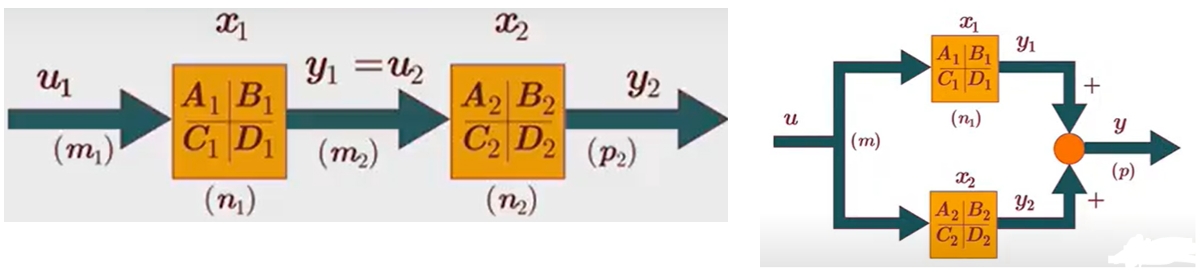
\includegraphics[scale = 0.6]{Figures/Electrical_connection}
		\caption{Mạch nối tiếp (trái) \& Mạch song song (phải)}
		\label{fig:electricalconnection}
	\end{figure}
	
	\noindent Giả sử rằng các hệ con đều là quan sát được. \\
	a) Chứng minh rằng nếu hệ thống tổng là quan sát được thì nó không thể có vector riêng trái dạng $w = \m{w_1 & 0} \in \C^{n_1+n_2}$ mà thỏa mãn điều kiện $w^H B= 0$ . \\
	b) Chứng minh hệ thống song song sẽ đánh mất tính quan sát được khi và chỉ khi $A_1$ và $A_2$ có giá trị riêng chung $\lambda$, và các vector riêng trái $w_1$, $w_2$ tương ứng thỏa mãn
	\begin{align*}
		& w^H_1 B_1 + w^H_2 B_2 = 0, \\
		& w^H_1 A_1 = \lambda w^H_1,   \   w^H_2 A_2 = \lambda w^H_2.
	\end{align*}
\end{bt}

\begin{bt}
	Mệnh đề sau có luôn luôn đúng không?
	%
	\[
	\rank \m{B & A B & \dots & A^{n-1}B} = \rank \m{AB & A^2 B & \dots & A^{n} B} \ .
	\]
	% 
	Nếu không, nó sẽ đúng với điều kiện nào?
\end{bt}

\begin{bt}
	Đối với hệ LTI, hãy chứng tỏ rằng $(A, B)$ là điều khiển được khi và chỉ khi $(-A, B)$ là điều khiển được. Điều này có đúng với các hệ thống LTV không?
\end{bt}   

\begin{bt}
	Hãy xét tính điều khiển được của các hệ điều khiển sau
	%
	\begin{equation}
		\dot{x} = \m{0 & 1 & 0 \\ 0 & 0 & 1 \\ 1 & -3 & -3} x + \m{0 \\ 0 \\ 1} u, \quad
		y = \m{1 & 2 & 1} x. 
	\end{equation}
\end{bt}
%
